\documentclass[a4paper, 11pt]{article}

\usepackage[colorlinks=true]{hyperref} % for cross-referencing, loads iftex for conditional statements

\ifPDFTeX	%using pdflatex compiler
\usepackage[utf8]{inputenc}
\usepackage[T1]{fontenc}
\else % using XeLateX or LuaLaTeX compiler - modern compilers supporting new fonts
\usepackage{fontspec}
\fi

\usepackage[left=2.54cm, right=2.54cm, top=2.54cm, bottom=2.54cm]{geometry}	% setting up page layout
\usepackage{graphicx}	% package to include figures
\usepackage{float} %pacakge to adjust figures/table positioning in doc
\usepackage{amsthm, amssymb, amsmath}	% math related packages; amsthm - theorem like environments, symb - for math fonts, math for multiline equations, matrices

\usepackage[dvipsnames, svgnames]{xcolor} % package to access different colors

\usepackage{tabularray} % new pacakage for tables - more robust compared to default tables in latex
\usepackage{mhchem} %for writing chemical eqns of formulas

% package fpr adding citations (bibliography)
\usepackage[style=numeric, 
			sorting=none,
			sortcites=true,
			maxbibnames=20,
			mincitenames=1,
			maxcitenames=2
			]{biblatex}
% style = output style for intext citations
% sorting - sorts the citation, default is name year title, but setting to none keep references in order in which they appear in text.
% sortcites - useful for multiple citations inside singel cite command. sorts them in numeric order.
% max/min citenames to control how many authors appear in text. with current options only main author name would appear in text e.g. J. Doe et al. 
% maxbibnames control the number of authors that would appear in the bibliography (end of document)

\usepackage{subcaption}	% support for subfigures
\usepackage{caption}	% customizing captions for float environments - not maintained anymore, but included here because of question regarding caption placement during last session.
%\captionsetup{justification=raggedright,singlelinecheck=false} % uncomment it to globally set the captions to start from left of page. singlelinecheck=false ensures that small captions do no start at center of page.


\usepackage{listings}	% for including source code in latex. 
% Alternatively `minted` can be used for source code, but that requires python installation.
\lstset{
	language=[LaTeX]TeX,
	keywordstyle=\color{red},
	commentstyle=\color{DarkGreen},
	stringstyle=\color{Purple},
	basicstyle=\small\ttfamily,
	backgroundcolor=\color{Gray!10},
	breaklines,
	numbers=left,
	breakatwhitespace=true,
	tabsize=2,
	morekeywords={includegraphics, textcolor, textsubscript, textsuperscript, listoffigures, part, chapter, subsection, subsubsection, paragraph, subparagraph, maketitle, tableofcontents, subfigure},
	literate={\$}{{\textcolor{teal}{\$}}}{1}
}

\usepackage{cleveref}	% for intelligent cross-referecning 

\setlength{\parindent}{0pt}	%sets amount of indentation added to first line of paragraph

%\crefname{lstlisting}{listing}{listings}
%\Crefname{lstlisting}{Listing}{Listings}

\graphicspath{{Figures/}}	%specifying location globally to avoid writing the whole path everytime

\author{Muhammad Qasim Riaz}
\title{Introduction to \LaTeX{}}
\date{\today}

\begin{document}
	
\maketitle %automatically creates a title page from metadata.

\tableofcontents

\newpage
	
\section{Document structure}\label{sec:Document-structure}
	
	\LaTeX document can be divided into three main parts;

	\begin{enumerate}
		\item Document class
		\item Preamble
		\item Document body
	\end{enumerate}
	
	\subsection{Document class}\label{sec:Document-class}
	
	This is the first line of \LaTeX document, and defines the type (or class) of document. Some of the common classes include:
	
	\begin{itemize}
		\item \texttt{article} $\rightarrow$ to write articles/short reports. Top level header is \lstinline|section| and from there it goes to \lstinline|subsection|, \lstinline|subsubsection| and so on.
		\item \texttt{book} $\rightarrow$ for books. Supports \lstinline|part| and \lstinline|chapter| levels for writing. And if I recall correctly, has different margins for odd/even pages.
		\item \texttt{beamer} $\rightarrow$ for creating presentations.
	\end{itemize}

	In addition to defining the type of document, the command \lstinline|\documentclass| also supports optional arguments. Some of the options are:
	
	\begin{itemize}
		\item papersize $\rightarrow$ a4, a5, letter etc.
		\item fontsize $\rightarrow$ font size are defined in terms of \emph{pt}. Default is 10pt.
		\item orientation $\rightarrow$ landscape/portrait. Default is portrait.
	\end{itemize}
	
	An example of document class is:
	
	\begin{lstlisting}[label={lst:class}, caption={Document class}]
\documentclass[a4paper, 10pt]{article}
	\end{lstlisting}
	
	\subsection{Preamble}\label{sec:Preamble}
	This section defines all the packages that are required for the document, settings that apply to whole document, user based commands (or macros) as well as document metadata. An example of preamble is presented in \Cref{lst:preamble}:
	
\begin{lstlisting}[label={lst:preamble}, caption={Definining document preamble}]
% packages
\usepackage[colorlinks=true]{hyperref} 
\usepackage[utf8]{inputenc}
\usepackage[T1]{fontenc}
\usepackage[left=2.54cm, right=2.54cm, top=2.54cm, bottom=2.54cm]{geometry}	

% settings for document
\setlength{\parindent}{0pt}	% set indentation from left at beginning of paragraph. 
\setcounter{tocdepth}{2}	% table of contents depth

% metadata
\author{names}
\title{text}
\date{text}
\end{lstlisting}
	
	\subsection{Document body}\label{sec:Document-body}
	This is the part where actual text (text that you want to put in document) goes. The contents are enclosed by \lstinline|\begin{document}| and \lstinline|\end{document}| commands. Inside document body, one can include different environments like figures, tables, equations and so on. 
	
	Some common formatting options:
	
	\begin{itemize}
		\item \lstinline|\textbf{Bold text}| $\rightarrow$ \textbf{Bold text}
		\item \lstinline|\textit{Italic text}| $\rightarrow$ \textit{Italic text}
		\item \lstinline|\underline{Underline text}| $\rightarrow$ \underline{Underline text} 
		\item \lstinline|A\textsubscript{subscript}| $\rightarrow$ A\textsubscript{subscript}
		\item \lstinline|A\textsubscript{subscript}| $\rightarrow$ A\textsuperscript{superscript}
		\item \lstinline|\textcolor{Blue}{blue text}|$\rightarrow$ \textcolor{Blue}{blue text}
		\item \lstinline|\newline| or \lstinline|\\| $\rightarrow$ for line break.
		\item \lstinline|\newpage| $\rightarrow$ forcing page break.
	\end{itemize}                               

	A simple example for document body is presented in \cref{lst:document-body}. The command \lstinline|\maketitle| generates a title from metadata as defined in \Cref{sec:Preamble}. The command \lstinline|\tableofcontents| produces table of contents (toc). By default toc depth is 3 for the article class, meaning headings upto and including \lstinline|\subsubsection{}| are included in the toc. This can be modified using \lstinline|\setcounter{tocdepth}{2}| in document preamble. In this particular example the depth is set to 2, meaning only \lstinline|\section{}| and \lstinline|\subsection{}| are included in toc.
	
	
\begin{lstlisting}[caption={Example for document body}, label={lst:document-body}]
\begin{document}
	
	\maketitle
	\tableofcontents
	\newpage
	
	\section{Introduction}
	
	\section{Material and methods}
	
	\subsection{Chemicals}
	
	\subsection{Analytical methods}
	
\end{document}
\end{lstlisting}
	
	\subsubsection{Section commands}
	In \LaTeX{} the document can be structured into chapters, section, subsection and so on. The nesting order is:
	
	\begin{enumerate}
		\item \lstinline|\part{}|
		\item \lstinline|\chapter{}|
		\item \lstinline|\section{}|
		\item \lstinline|\subsection{}|
		\item \lstinline|\subsubsection{}|
		\item \lstinline|\paragraph{}|
		\item \lstinline|\subparagraph{}|
	\end{enumerate}
	
	In \lstinline|\documentclass{article}| the top level heading is \lstinline|\section{}| and \lstinline|\part{}| or \lstinline|\chapter{}| throws an error. Those levels are available in book or report class.
	
	In addition, there are also commands with asterik (*) at their end. This suppresses the numbering and exclude the header from table of contents. See
	
\section{Equation}

Writing equation in \LaTeX is very simple. Equations can be written in line using \$ operator, or they can be written inside math environment. See \cref{lst:equations} for example

\begin{lstlisting}[caption={Writing equations in \LaTeX}, label={lst:equations}]
Equations can be written inline e.g. Relativity states $E=mc^{2}$

Equation can also be written in display mode using the \texttt{equation} environment:
\begin{equation}
	E = mc^{2}
\end{equation}
\end{lstlisting}

Equations can be written inline e.g. Relativity states $E=mc^{2}$

Equation can also be written in display mode using the \texttt{equation} environment:
\begin{equation}
	E = mc^{2}
\end{equation}

Spacing is ignored in math mode. To add space between characters or operators use backslash (\textbackslash) followed by space.

\subsection{Sub-equations}
\LaTeX{} also supports writing sub-equations (\cref{lst:subequations}). Writing math characters\footnote{For a full list of \LaTeX{} symbols see \href{https://www.texlive.info/CTAN/info/symbols/comprehensive/symbols-a4.pdf}{The Comprehensive LATEX Symbol List}} is also quite intuitive, normally the character is preceded by a backslash (\textbackslash) e.g. \lstinline|$\rho$| $\rightarrow$ $\rho$. Note that for writing Greek/Latin characters within text requires the same syntax as inline equations, i.e. enclosing it between \$ operator. Few more things to note in \cref{lst:subequations};
\begin{itemize}
	\item the command \lstinline|label{key}| is used to create an anchor for cross-referencing the object at some other point in document.
	\item Math (or equation environment) normally writes everything in \emph{italics}. \lstinline|$\mathrm{}$| formats the math symbols to normal (roman) font. 
	\item Simple operators like addition and subtraction can be written as keyboard characters (+ or -). For multiplication use \lstinline|\times or \cdot| $\rightarrow$ $\times$ or $\cdot$ respectively. For division, use \lstinline|$\frac{num}{den}$| $\rightarrow$ $\frac{num}{den}$
\end{itemize} 

\begin{lstlisting}[caption={Writing subequations}, label={lst:subequations}]
\begin{subequations}
\begin{gather}
\mathrm{uc_{f}|_{z = 0} = uc_f|_{z = 0^+} - D_{ax}\frac{\partial c_f}{\partial z}\Bigg|_{z = 0^+}} \label{eq:BC-inlet} \\
\mathrm{\frac{\partial c_f(z = L, t)}{\partial z} = 0} \label{eq:BC-outlet} 
\end{gather}
\label{eq:BoundaryConditions}
\end{subequations}
\end{lstlisting}

\begin{subequations}
	\begin{gather}
		\mathrm{uc_{f}|_{z = 0} = uc_f|_{z = 0^+} - D_{ax}\frac{\partial c_f}{\partial z}\Bigg|_{z = 0^+}} \label{eq:BC-inlet} \\
		\mathrm{\frac{\partial c_f(z = L, t)}{\partial z} = 0} \label{eq:BC-outlet} 
	\end{gather}
	\label{eq:BoundaryConditions}
\end{subequations}

\subsection{Multiline equations}
Sometimes the equations are too long to be properly displayed on a single line. In that case use \texttt{split} or \texttt{multiline} environment to write multiline equations with predefined line breaks. See \cref{lst:multiline-equation} for code, and \cref{eq:multiline,eq:align} for ´output.

\begin{lstlisting}[caption={Writing multiline equations in \LaTeX{}}, label={lst:multiline-equation}]
\begin{multline}
	\mathrm{\frac{\partial c}{\partial t} =  - u\cdot\frac{c_{i+1,j} - c_{i-1,j}}{2\Delta x} - v \cdot \frac{c_{i,j+1} - c_{i,j-1}}{2\Delta y}} \\
	\mathrm{+ \mathbb{D} \left(\frac{c_{i+1,j} - 2c_{i,j} + c_{i-1,j}}{\Delta x^{2}} + \frac{c_{i,j+1} - 2c_{i,j} + c_{i,j-1}}{\Delta y^{2}} \right) + R}
	\label{eq:multiline}
\end{multline}	

\begin{equation}
	\begin{split}
		\mathrm{p(\theta|y,n)\ } & \propto \mathrm{\theta^{y} (1-\theta)^{n-y} \theta^{\alpha-1} (1-\theta)^{\beta - 1}} \\
		& \propto \mathrm{\theta^{y + \alpha - 1} (1-\theta)^{n - y + \beta - 1} } \\
		& \propto \mathrm{Beta(\alpha+y, \beta+n-y)}
		\label{eq:align}
	\end{split}
\end{equation}
\end{lstlisting}

\begin{multline}
	\mathrm{\frac{\partial c}{\partial t} =  - u\cdot\frac{c_{i+1,j} - c_{i-1,j}}{2\Delta x} - v \cdot \frac{c_{i,j+1} - c_{i,j-1}}{2\Delta y}} \\
	 \mathrm{+ \mathbb{D} \left(\frac{c_{i+1,j} - 2c_{i,j} + c_{i-1,j}}{\Delta x^{2}} + \frac{c_{i,j+1} - 2c_{i,j} + c_{i,j-1}}{\Delta y^{2}} \right) + R}
	 \label{eq:multiline}
\end{multline}	

\begin{equation}
\begin{split}
	\mathrm{p(\theta|y,n)\ } & \propto \mathrm{\theta^{y} (1-\theta)^{n-y} \theta^{\alpha-1} (1-\theta)^{\beta - 1}} \\
	& \propto \mathrm{\theta^{y + \alpha - 1} (1-\theta)^{n - y + \beta - 1} } \\
	& \propto \mathrm{Beta(\alpha+y, \beta+n-y)}
	\label{eq:align}
\end{split}
\end{equation}



\section{Figures}

Figures in \LaTeX{} are included using \texttt{figure} environment. The supported types are \texttt{.pdf, .eps, .png, .jpeg}. General syntax for including figures is given in \cref{lst:figures}. Important to include packages \texttt{graphicx} and \texttt{float} in document preamble. The latter is required for changing figure position.

\begin{lstlisting}[caption={Including figures in \LaTeXe}, label={lst:figures}]
\begin{figure}[H]
\centering
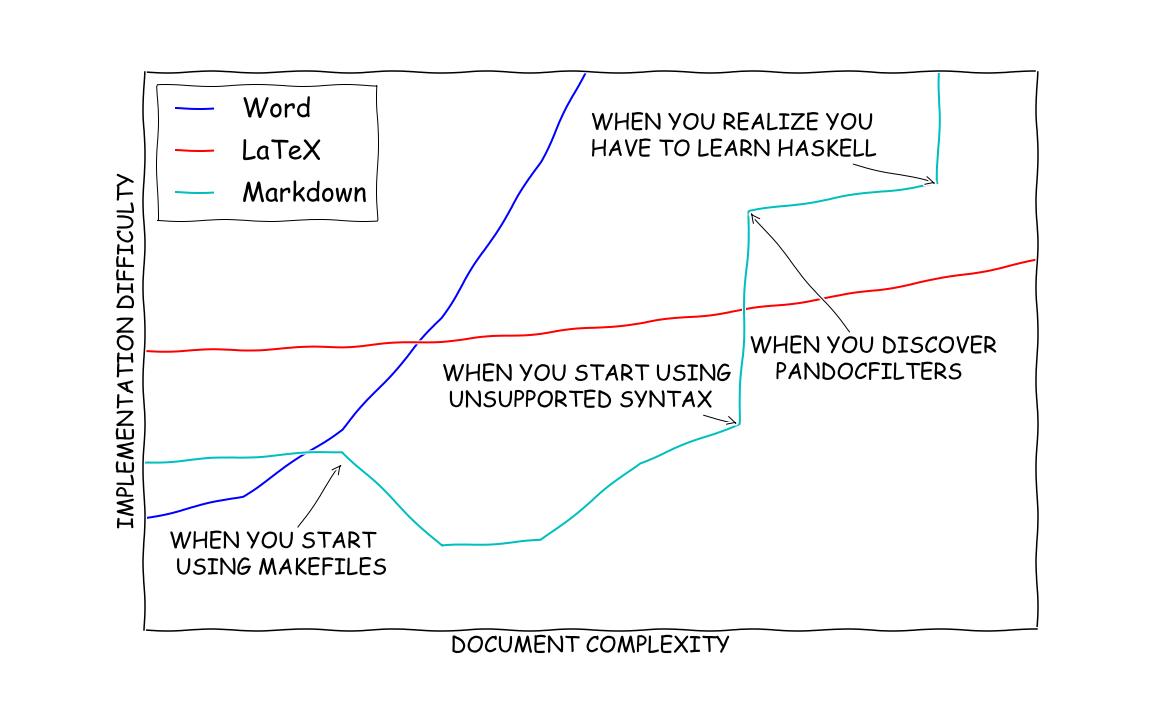
\includegraphics[width=0.6\textwidth]{learning_curve.png}
\caption[Comparison between different tools for writing text]{Comparison between different tools for writing text. \LaTeX{} is a bit difficult to start with, but becomes easier to write with time. Markdown is also a nice way of writing documents. See \href{https://quarto.org/docs/authoring/markdown-basics.html}{Quarto} for a good markdown option.}
\label{fig:demo_figure}
\end{figure}
\end{lstlisting}

\begin{figure}[H]
	\centering
	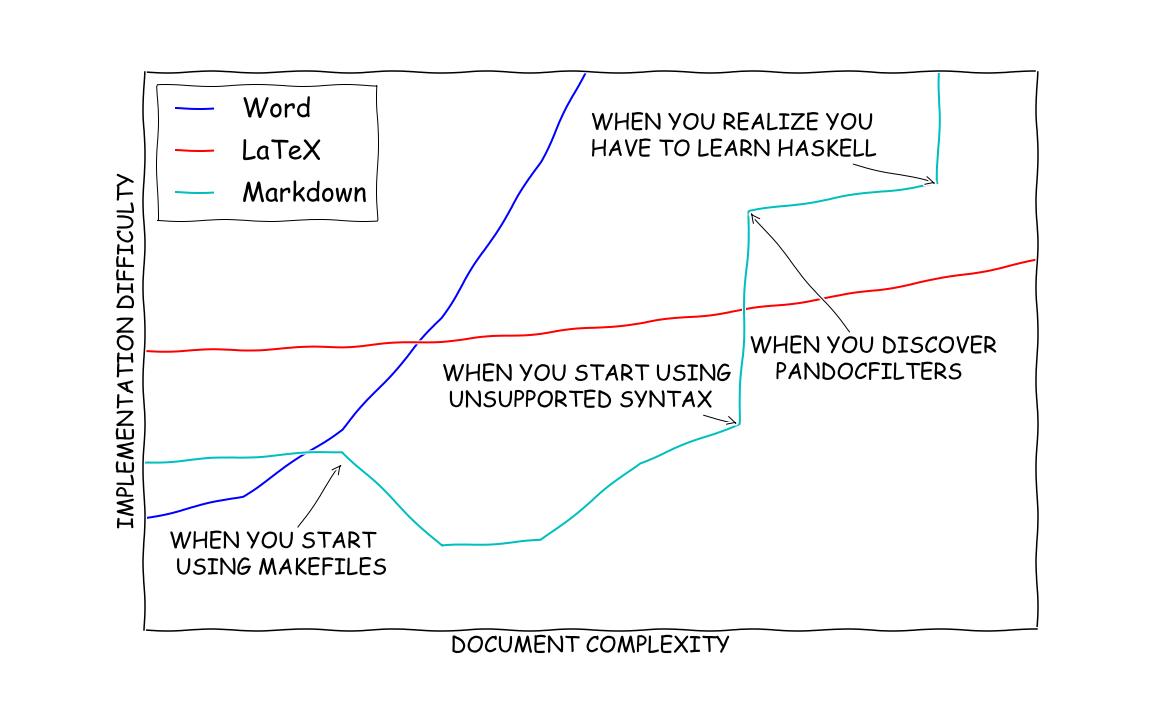
\includegraphics[width=0.6\textwidth]{learning_curve.png}
	\caption[Comparison between different tools for writing text]{Comparison between different tools for writing text. \LaTeX{} is a bit difficult to start with, but becomes easier to write with time. Markdown is also a nice way of writing documents. See \href{https://quarto.org/docs/authoring/markdown-basics.html}{Quarto} for a good markdown option.}
	\label{fig:demo_figure}
\end{figure}

Some notes for \cref{lst:figures}; 
\begin{itemize}
	\item \lstinline|[H]| right after figure environment tells the compiler to place figure precisely at that point. Other options include \texttt{t}; page top, \texttt{b}; page bottom, \texttt{h}; approximately here.
	\item \lstinline|\centering| is used to instruct the compile to horizontally center figure.
	\item \lstinline|\includegraphics| is the command that actually includes the figure. The argument in \lstinline|[]| are optional. There are several options including some for trimming the figure, but normally I only use sizing (width) argument. In my experience, cropping the figure or removing white spaces in figures is more easy using external tools like adobe or inkscape.
	\item \lstinline|caption| command has two arguments:
		\begin{itemize}
			\item \lstinline|[short caption]| - optional argument that appears in list of figures if included in document. List of figures can be generated using command \lstinline|\listoffigures| inside document body.
			\item \lstinline|{long caption}| - required argument, which appears below the figure.
		\end{itemize}
	\item \lstinline|\label{key}| to create anchor for cross-referencing. 
\end{itemize}

\subsection{Subfigures}
Often one wants to include multiple figures in a panel layout. This can be easily done using the \lstinline|subfigure| environment which requires loading the \texttt{subcaption} package in preamble. See \cref{lst:subfigures} for source code for \Cref{fig:Neural-Network-Activation-Functions}. Captions and labels can be provided individually for each subfigure. e.g. \lstinline|\Cref{fig:ReLU-Function}| $\rightarrow$ \Cref{fig:ReLU-Function}.

In \cref{lst:subfigures}, each subfigure is assigned a fixed width upfront e.g. \lstinline|\begin{subfigure}{0.49\textwidth}| tells the compiler to use 49\% of available textwidth for that figure. One can also use \lstinline|\linewidth|, but this may cause the figure to extend beyond normal text margins.

\begin{figure}[H]
	\centering
	\begin{subfigure}{0.49\textwidth}
		\centering
		\includegraphics[width=\textwidth]{ReLU.pdf}
		\caption{Rectified linear unit (ReLU) function}
		\label{fig:ReLU-Function}
	\end{subfigure}
	\hfill
	\begin{subfigure}{0.49\textwidth}
		\centering
		\includegraphics[width=\textwidth]{SIGMOID.pdf}
		\caption{Sigmoid function}
		\label{fig:Sigmoid-Function}
	\end{subfigure}
	\begin{subfigure}{0.49\textwidth}
		\centering
		\includegraphics[width=\textwidth]{SIGN.pdf}
		\caption{Sign function}
		\label{fig:Sign-Function}
	\end{subfigure}
	\hfill
	\begin{subfigure}{0.49\textwidth}
		\centering
		\includegraphics[width=\textwidth]{TANH.pdf}
		\caption{Hyperbolic tangent function}
		\label{fig:Tanh-Function}
	\end{subfigure}
	\caption{Some commonly used activation functions for neural networks}
	\label{fig:Neural-Network-Activation-Functions}
\end{figure}

\begin{lstlisting}[caption={Creating subfigures in \LaTeX{}}, label={lst:subfigures}]
\begin{figure}[H]
	\centering
	\begin{subfigure}{0.49\textwidth}
		\centering
		\includegraphics[width=\textwidth]{ReLU.pdf}
		\caption{Rectified linear unit (ReLU) function}
		\label{fig:ReLU-Function}
	\end{subfigure}
	\hfill
	\begin{subfigure}{0.49\textwidth}
		\centering
		\includegraphics[width=\textwidth]{SIGN.pdf}
		\caption{Sign function}
		\label{fig:Sign-Function}
	\end{subfigure}

	\begin{subfigure}{0.49\textwidth}
		\centering
		\includegraphics[width=\textwidth]{SIGMOID.pdf}
		\caption{Sigmoid function}
		\label{fig:Sigmoid-Function}
	\end{subfigure}
	\hfill
	\begin{subfigure}{0.49\textwidth}
		\centering
		\includegraphics[width=\textwidth]{TANH.pdf}
		\caption{Hyperbolic tangent function}
		\label{fig:Tanh-Function}
	\end{subfigure}
	\caption{Some commonly used activation functions for neural networks}
	\label{fig:Neural-Network-Activation-Functions}
\end{figure}
\end{lstlisting}

\subsection{Caption alignment}
By default captions are centered in \LaTeX{}. However one can change them to left or right using the commands listed in \cref{lst:caption-alignment} (\Cref{fig:Left-caption}). This requires loading \texttt{caption} package to be loaded in preamble. For right alignment one can replace \lstinline|raggedright| with \lstinline|raggedleft|. Notice that the \lstinline|\captionsetup{}| is specified within the \lstinline|figure| environment, so only the caption for this figure will be affected. To avoid repeating this for every figure, use the same command in document preamble after loading the caption package.

\begin{lstlisting}[caption={Figure caption alignment}, label={lst:caption-alignment}]
\begin{figure}[H]
	\captionsetup{justification=raggedright,singlelinecheck=false}
	\centering
	\includegraphics[width=0.6\textwidth]{ReLU.pdf}
	\caption{Left aligned captions}
	\label{fig:Left-caption}
\end{figure}
\end{lstlisting}

\begin{figure}[H]
	\captionsetup{justification=raggedright,singlelinecheck=false}
	\centering
	\includegraphics[width=0.6\textwidth]{ReLU.pdf}
	\caption{Left aligned captions}
	\label{fig:Left-caption}
\end{figure}

\section{Tables}
Default tables in \LaTeX{} don't require any package. However, they are limited in their output. For this reason we use the \texttt{tabularray} package, that provides support for long tables as well as other useful functionalities. An example of long table generated using \texttt{tabularray} is provided in 

\begin{lstlisting}[caption={Using \texttt{longtblr} from \texttt{tabularray} for tables}, label = {lst:longtables}]
\begin{longtblr}
	[
		caption={Commonly used activation functions for neural networks},
		label={tab:ActivationFcns}
	]
	{
		colspec={|[2pt]X[4cm,m,j]|X[3.5cm,m,c]|X[4cm,m,c]|[2pt]},
		rowhead={1},
		row{1} = gray4,
		hline{1,Z}={2pt},
		hline{2-Y}={1pt}
	}
	\textcolor{white}{\textbf{Activation Function}} & \textcolor{white}{\textbf{Equation}} & \textcolor{white}{\textbf{Graphical representation}} \\
	Sigmoid function & \SetCell{mode=dmath} \phi(x) = \frac{1}{1+e^{-x}} & \begin{minipage}{\linewidth}
		\includegraphics[width=\textwidth]{Figures/SIGMOID}
	\end{minipage}\\
	Hyperbolic tangent function & \SetCell{mode=dmath} \phi(x)=\frac{2}{1+e^{-2x}}-1 & \begin{minipage}{\linewidth}
		\includegraphics[width=\textwidth]{Figures/TANH}
	\end{minipage} \\
	Rectified linear unit (ReLU) function & \SetCell{mode=dmath} \phi(x) = \max(0,x) & \begin{minipage}{\linewidth}
		\includegraphics[width=\textwidth]{Figures/ReLU}
	\end{minipage} \\
	Sign function & \SetCell{mode=dmath} \phi(x) = sign(x) & \begin{minipage}{\linewidth}
		\includegraphics[width=\textwidth]{Figures/SIGN}
	\end{minipage}
\end{longtblr}	
\end{lstlisting}

\begin{longtblr}
	[
		caption={Commonly used activation functions for neural networks},
		label={tab:ActivationFcns}
	]
	{
		colspec={|[2pt]X[4cm,m,j]|X[3.5cm,m,c]|X[4cm,m,c]|[2pt]},
		rowhead={1},
		row{1} = gray4,
		hline{1,Z}={2pt},
		hline{2-Y}={1pt}
	}
	\textcolor{white}{\textbf{Activation Function}} & \textcolor{white}{\textbf{Equation}} & \textcolor{white}{\textbf{Graphical representation}} \\
	Sigmoid function & \SetCell{mode=dmath} \phi(x) = \frac{1}{1+e^{-x}} & \begin{minipage}{\linewidth}
		\includegraphics[width=\textwidth]{Figures/SIGMOID}
	\end{minipage}\\
	Hyperbolic tangent function & \SetCell{mode=dmath} \phi(x)=\frac{2}{1+e^{-2x}}-1 & \begin{minipage}{\linewidth}
		\includegraphics[width=\textwidth]{Figures/TANH}
	\end{minipage} \\
	Rectified linear unit (ReLU) function & \SetCell{mode=dmath} \phi(x) = \max(0,x) & \begin{minipage}{\linewidth}
		\includegraphics[width=\textwidth]{Figures/ReLU}
	\end{minipage} \\
	Sign function & \SetCell{mode=dmath} \phi(x) = sign(x) & \begin{minipage}{\linewidth}
		\includegraphics[width=\textwidth]{Figures/SIGN}
	\end{minipage} \\
\end{longtblr}


\end{document}
